
\documentclass{article}
\usepackage[utf8]{inputenc}
\usepackage{relsize}
\usepackage{amsmath}
\usepackage{geometry}
\usepackage{tikz}
\usetikzlibrary{automata, positioning, arrows}
\tikzset{node distance=2.5cm, % Minimum distance between two nodes. Change if necessary.
every state/.style={ % Sets the properties for each state
semithick,
fill=gray!10},
initial text={}, % No label on start arrow
double distance=2pt, % Adjust appearance of accept states
every edge/.style={ % Sets the properties for each transition
draw,->,>=stealth', % Makes edges directed with bold arrowheads
auto,semithick}}

\geometry{
 a4paper,
 total={170mm,257mm},
 left=20mm,
 top=20mm,
}

\title{Homework 2\\[0.2em]\smaller{}CSC 445-01: Theory of Computation}
\author{Matthew Mabrey, Luke Kurlandski}
\date{\today}

\begin{document}

\maketitle

\section*{1.12}

We describe $D$ more simply
$$D = \{w \big | w \textrm{  is a word with an odd number of } b \textrm{'s followed by an even number of } a \textrm{'s} \}$$
And construct a DFA that recognizes $D$
\begin{center}
    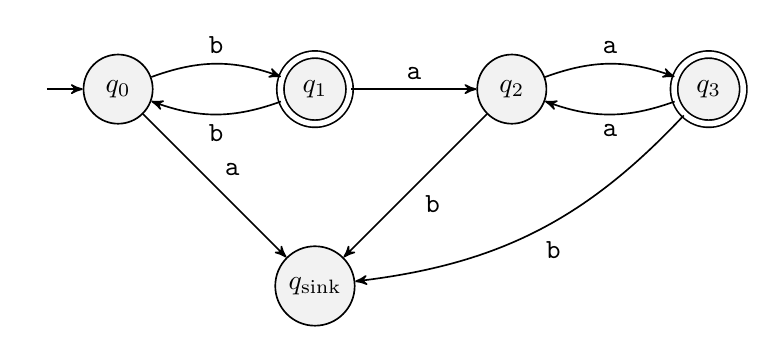
\begin{tikzpicture}
    
    \node[state, initial] (0) {$q_0$};
    \node[state, right of=0, accepting] (1) {$q_1$};
    \node[state, right of=1] (2) {$q_2$};
    \node[state, right of=2, accepting] (3) {$q_3$};
    \node[state, below of=1] (4) {$q_\textrm{sink}$};
    
    \draw (0) edge[bend left=20] node {\tt b} (1);
    \draw (1) edge[bend left=20] node {\tt b} (0);
    \draw (1) edge node {\tt a} (2);
    \draw (2) edge[bend left=20] node {\tt a} (3);
    \draw (3) edge[bend left=20] node {\tt a} (2);
    
    \draw (0) edge node {\tt a} (4);
    \draw (2) edge node {\tt b} (4);
    \draw (3) edge[bend left=20] node {\tt b} (4);
    
    \end{tikzpicture}
\end{center}

\section*{1.20 g}

For the regular expression $R = (\epsilon \cup a)b $\\\\
Members include
\begin{itemize}
    \item $b$
    \item $ab$
\end{itemize}
Non members include
\begin{itemize}
    \item $a$
    \item $aba$
\end{itemize}

\section*{1.40 b}

Suppose the language $A$ is regular. Then we can construct an NFA $N$ that recognizes $A$. We can apply a simple modification to $N$ to have it recognize $\textrm{NoExtend(A)}$. Since $\textrm{NoExtend(A)}$ is recognized by an NFA, lets call it $N'$, it is regular. Therefore, the class of regular languages is closed under the $\textrm{NoExtend()}$ operation.\\\\
Given the NFA $N = (Q, \Sigma, \delta, q_0, F)$ that recognizes $A$, we construct $N' = (Q', \Sigma', \delta', q_0', F')$ that recognizes $\textrm{NoExtend(A)}$ where 
\begin{itemize}
    \item $Q' = Q \cup \{q_f\}$ : we add one additional state to $Q$ and make it the one and only final state.
    \item $\Sigma' = \Sigma$ : we keep the same alphabet.
    \item $\delta' = \delta \cup \delta_\textrm{new}$ : we keep all of the old transitions but add some new ones. Out of every state, we add a arrow for every letter in $\Sigma$ that the state did not already have leaving it. This arrow then leads to $q_f$. This causes the automata to enter the accept state as soon as it reads a character that confirms the string is not a substring of any word accepted by $N$.
    \item $q_0' = q_0$ : we keep the same start state
    \item $F' = \{q_f\}$ : we make the set of accept states our new state.
\end{itemize}

\end{document}
